\documentclass[12pt,pdflatex]{elsarticle} 

%%%%%%%%%%%%%%%%%%%%%%%%%%%%%%%%%%%%%%%%%%%%%%%%%%
%%%%%%%%%%%%%%%%%%%% PREAMBLE %%%%%%%%%%%%%%%%%%%%
%%%%%%%%%%%%%%%%%%%%%%%%%%%%%%%%%%%%%%%%%%%%%%%%%%


% -------------------- defaults -------------------- %
% load lots o' packages

% references
\usepackage{natbib}

% Fonts
\usepackage[default,osfigures,scale=0.95]{opensans}
\usepackage[T1]{fontenc}
\usepackage{ae}
% to colorize links in document. See color specification below
\usepackage[pdftex,hyperref,x11names]{xcolor}
% load the hyper-references package and set document info
\usepackage[pdftex]{hyperref}

% Generate some fake text
\usepackage{blindtext}

% layout control
\usepackage{geometry}
\geometry{verbose,tmargin=1.25in,bmargin=1.25in,lmargin=1.1in,rmargin=1.1in}
\usepackage{parallel}
\usepackage{parcolumns}
\usepackage{fancyhdr}

% math typesetting
\usepackage{array}
\usepackage{amsmath}
\usepackage{amssymb}
\usepackage{amsfonts}
\usepackage{relsize}
\usepackage{mathtools}
\usepackage{bm}
\usepackage[%
decimalsymbol=.,
digitsep=fullstop
]{siunitx}

% restricts float objects to be inserted before end of section
% creates float barriers
\usepackage[section]{placeins}

% tables
\usepackage{tabularx}
\usepackage{booktabs}
\usepackage{multicol}
\usepackage{multirow}
\usepackage{longtable}

% to adapt caption style
\usepackage[font={small},labelfont=bf]{caption}

% footnotes at bottom
\usepackage[bottom]{footmisc}
   \renewcommand{\footnotelayout}{\doublespacing} % set spacing in footnotes
   \newlength{\myfootnotesep}
   \setlength{\myfootnotesep}{\baselineskip}
   \addtolength{\myfootnotesep}{-\footnotesep}
   \setlength{\footnotesep}{\myfootnotesep} % set spacing between footnotes

% to change enumeration symbols begin{enumerate}[(a)]
\usepackage{enumerate}

% to make enumerations and itemizations within paragraphs or
% lines. f.i. begin{inparaenum} for (a) is (b) and (c)
\usepackage{paralist}

% graphics stuff
\usepackage{subfig}
\usepackage{graphicx}
\usepackage[space]{grffile} % allows us to specify directories that have spaces
\usepackage{placeins} % prevents floats from moving past a \FloatBarrier
\usepackage{tikz}
\usepackage{rotating}

% Spacing
\usepackage[doublespacing]{setspace}

% -------------------------------------------------- %


% -------------------- page template -------------------- %

\setlength{\headheight}{15pt}
\setlength{\headsep}{20pt}
\pagestyle{fancyplain}
 
\fancyhf{}
 
\lhead{\fancyplain{}{}}
\chead{\fancyplain{}{Amen for LFM}}
\rhead{\fancyplain{}{\today}}
\rfoot{\fancyplain{}{\thepage}}

% ----------------------------------------------- %


% -------------------- customizations -------------------- %

% easy commands for number propers
\newcommand{\first}{$1^{\text{st}}$}
\newcommand{\second}{$2^{\text{nd}}$}
\newcommand{\third}{$3^{\text{rd}}$}
\newcommand{\nth}[1]{${#1}^{\text{th}}$}

% easy command for boldface math symbols
\newcommand{\mbs}[1]{\boldsymbol{#1}}

% command for R package font
\newcommand{\pkg}[1]{{\fontseries{b}\selectfont #1}}

% approx iid
\newcommand\simiid{\stackrel{\mathclap{\normalfont\mbox{\tiny{iid}}}}{\sim}}

% -------------------------------------------------------- %

%%%%%%%%%%%%%%%%%%%%%%%%%%%%%%%%%%%%%%%%%%%%%%%%%%
%%%%%%%%%%%%%%%%%%%% DOCUMENT %%%%%%%%%%%%%%%%%%%%
%%%%%%%%%%%%%%%%%%%%%%%%%%%%%%%%%%%%%%%%%%%%%%%%%%

% remove silly elsevier preprint note
\makeatletter
\def\ps@pprintTitle{%
 \let\@oddhead\@empty
 \let\@evenhead\@empty
 \def\@oddfoot{}%
 \let\@evenfoot\@oddfoot}

\def\input@path{{/Users/janus829/Dropbox/Research/netModels/summResults/}, {/Users/s7m/Dropbox/Research/netModels/summResults/}, {/Users/mdw/Dropbox/netModels/summResults/}}
\graphicspath{{/Users/janus829/Dropbox/Research/netModels/summResults/}, {/Users/s7m/Dropbox/Research/netModels/summResults/},{/Users/mdw/Dropbox/netModels/summResults/}}
\makeatother

\begin{document}

% % saying hello ----------------------------------------------- %
% \thispagestyle{empty}
% \begin{frontmatter}
%
% \title{Inferential Approaches for Network Analysis: \\ AMEN for Latent Factor Models\tnoteref{t1}}
%
% \tnotetext[t1]{This research was partially supported by the National Science Foundation Award 1259266.}
%
% \author[msu]{Shahryar Minhas\corref{cor1}}
% \ead{minhassh@msu.edu}
% \cortext[cor1]{Corresponding author}
% \author[duke2]{Peter D. Hoff}
% \author[duke]{Michael D. Ward}
%
% \address[msu]{Department of Political Science, Michigan State University, East Lansing, MI 48824, USA}
% \address[duke]{Department of Political Science, Duke University, Durham, NC 27701, USA}
% \address[duke2]{Departments of Statistics, Duke University, Durham, NC 27701, USA}
%
% \begin{abstract}
% There is growing interest in the study of social networks enabling  scholars to move away from focusing on individual observations to examining more precisely the interrelationships among observations. Many network approaches have been developed in a descriptive fashion, but attention to inferential approaches using statistical models of networks has been growing. We review a latent factor approach that models interdependencies among observations using additive and multiplicative effects (AME) which can be applied to binary, ordinal, and continuous network data. We compare  this to alternative latent variable models as well as to exponential random graph models (ERGM). The AME approach can be easily implemented in the context of general linear models. It is both computationally straightforward and avoids degeneracy, which often plagues ERGM. In an out-of-sample context, it out-performs alternatives in terms of predicting links and capturing network dependencies.
% \end{abstract}
% \end{frontmatter}
%
% % ----------------------------------------------- %

\newpage\setcounter{page}{1} 

Network analysis provides a way to represent and study ``relational data'', that is data with characteristics extending beyond those of the individual, or in the parlance of International Relations (IR), characteristics beyond the monadic level. Data structures that extend beyond the monadic level are quite simply the norm when it comes to the study of events such as trade, interstate conflict, or the formation of international agreements. The dominant paradigm in  international relations for dealing with such data structures, however, is not a network approach but rather a dyadic design, in which an interaction between a pair of countries is considered independent of interactions between any other pair in the system.\footnote{To highlight the ubiquity of this approach the following represent just a sampling of the articles published from the 1980s to the present in the American Journal of Political Science (AJPS) and American Political Science Review (APSR) that assume dyadic independence: \citet{dixon:1983,mansfield:etal:2000,lemke:reed:2001a,mitchell:2002,dafoe:2011a,fuhrmann:sechser:2014,carnegie:2014}.} 

The implication of this assumption is that when, for example, Vietnam and the United States decide to form a trade agreement, they make this decision independently of what they have done with other countries and what other countries in the international system have done among themselves.\footnote{There has been plenty of work done on treaty formation that would challenge this claim, e.g., see \citet{manger:etal:2012,kinne:2013}.} An even stronger assumption is that Japan declaring war against the United States is independent of the decision of the United States to go to war against Japan.\footnote{\citet{maoz:etal:2006,ward:etal:2007,minhas:etal:2016} would each note the importance of taking into account network dynamics in the study of interstate conflict.} A common refrain from those that favor the dyadic approach is that many events are only bilateral (\citealt{diehl:wright:2016}), thus alleviating the need for an approach that incorporates interdependencies between observations. This is clearly wrong. The network perspective asserts that even bilateral events and processes take place within a broader system. What takes place in one part of the system may be dependent upon events in another. At a minimum, we don't know whether independence of events and processes characterizes what we observe. We should at least examine this assertion.  

In this article, we introduce the additive and multiplicative effects (AME) model.\footnote{The AME approach has been developed into an $\sf{R}$ package named \pkg{amen} and is available on CRAN (\citealt{amenpkg}).} The AME approach to network modeling is a flexible framework that can be used to estimate many different types of cross-sectional and longitudinal networks with binary, ordinal, or continuous edges in a straightforward way. The AME modeling framework can provide a flexible and easy to use scheme through which scholars can study relational data. It addresses the issue of interdependence while still allowing scholars to examine theories that may only be relevant in the monadic or dyadic level. Further, at the network level it accounts for nodal and dyadic dependence patterns, and provides a descriptive visualization of higher-order dependencies such as homophily and stochastic equivalence. 

To highlight the differences between AME and alternative approaches for conducting statistical inference on networks, we examine a cross-sectional network measuring collaborations during the policy design of the Swiss CO$_{2}$ act. We show that AME provides a superior goodness of fit to the data in terms of ability to predict linkages and capture network dependencies. 
\\

\section*{\textbf{Addressing Dependencies in Dyadic Data}}

% {\large\sffamily\bfseries{Addressing Dependencies in Dyadic Data}} 
% \vspace{0.5em}

Relational, or dyadic, data provide measurements of how pairs of actors relate to one another. The easiest way to organize such data is the directed dyadic design in which the unit of analysis is some set of $n$ actors that have been paired together to form a dataset of directed dyads. 
Operationally, this type of data structure is represented as a $n \times n$ matrix, $\mathbf{Y}$, where the diagonals are typically undefined. The $ij^{th}$ entry defines the relationship sent from $i$ to $j$ and can be continuous or discrete.
%A tabular design such as this for a set of $n$ actors, $\{i, j, k\}$ results in $n \times (n-1)$ observations, denoted
%$Y_{ij}$, typically with values on the diagonal being undefined (or missing).
%as shown in Table~\ref{tab:netDesign}. 

%\begin{table}[ht]
%	\centering
%		\centering
%		\setlength{\tabcolsep}{10pt}
%		\caption{Structure of datasets used in canonical design.} 	%	
%		\begin{tabular}{ccc}
%			Sender & Receiver & Event \\
%			\hline\hline
%			$i$ & $j$ & $y_{ij}$ \\
%			\multirow{2}{*}{\vdots} & $k$ & $y_{ik}$ \\
%			~ & $l$ & $y_{il}$ \\
%			$j$ & $i$ & $y_{ji}$ \\
%			\multirow{2}{*}{\vdots} & $k$ & $y_{jk}$ \\
%			~ & $l$ & $y_{jl}$ \\
%			$k$ & $i$ & $y_{ki}$ \\
%			\multirow{2}{*}{\vdots} & $j$ & $y_{kj}$ \\
%			~ & $l$ & $y_{kl}$ \\
%			$l$ & $i$ & $y_{li}$ \\
%			\multirow{2}{*}{\vdots} & $j$ & $y_{lj}$ \\
%			~ & $k$ & $y_{lk}$ \\
%			\hline\hline
%		\end{tabular}
%		\label{tab:canDesign}
%\end{table}        

%\begin{table}[ht]
%		\centering
%		\setlength{\tabcolsep}{10pt}
%		\renewcommand{\arraystretch}{1.5}
%		\caption{A matrix representation of dyadic data. Senders are represented by the rows and receivers by the columns.}		
%		\begin{tabular}{c||cccc}
%		~ & $i$ & $j$ & $k$ & $l$ \\ \hline\hline
%		$i$ & \footnotesize{NA} & $y_{ij}$ & $y_{ik}$ & $y_{il}$ \\
%		$j$ & $y_{ji}$ & \footnotesize{NA}  & $y_{jk}$ & $y_{jl}$ \\
%		$k$ & $y_{ki}$ & $y_{kj}$ & \footnotesize{NA}  & $y_{kl}$ \\
%		$l$ & $y_{li}$ & $y_{lj}$ & $y_{lk}$ & \footnotesize{NA}  \\
%		\end{tabular}
%		\label{tab:netDesign}
%\end{table}

When modeling relational data, scholars typically employ a linear or generalized linear model (GLM). An assumption we make when applying this modeling technique is that each of the dyadic observations is conditionally independent on observed regressors. However, this is a strong assumption to make given that events between actors in a network are often interdependent. 
%The dependencies that tend to develop in relational data can be more easily understood when we move away from stacking dyads on top of one another and turn instead to a matrix design as illustrated in Table~\ref{tab:netDesign}.  
%Operationally, this type of data structure is represented as a $n \times n$ matrix, $\mathbf{Y}$, where the diagonals are typically undefined. The $ij^{th}$ entry defines the relationship sent from $i$ to $j$ and can be continuous or discrete.%Relations between actors in a network setting at times does not involve senders and receivers. Networks such as these are referred to as undirected and all the relations between actors are symmetric, meaning $y_{ij}=y_{ji}$.

The most common type of dependency that arises in networks are first-order, or nodal dependencies, and these point to the fact that we typically find significant heterogeneity in activity levels across nodes. The implication of this across-node heterogeneity is within-node homogeneity of ties, meaning that values across a row, say $\{y_{ij},y_{ik},y_{il}\}$, will be more similar to each other than other values in the adjacency matrix because each of these values has a common sender $i$. This type of dependency manifests in cases where sender $i$ tends to be more active or less active in the network than other senders. Similarly, while some actors may be more active in sending ties to others in the network, we might also observe that others are more popular targets, this would manifest in observations down a column, $\{y_{ji},y_{ki},y_{li}\}$, being more similar. Last, we might also find that actors who are more likely to send ties in a network are also more likely to receive them, meaning that the row and column means of an adjacency matrix may be correlated. Another ubiquitous type of structural interdependency is reciprocity. This is a second-order, or dyadic, dependency relevant only to directed datasets, and asserts that values of $y_{ij}$ and $y_{ji}$ may be statistically dependent. The prevalence of these types of potential interactions within directed dyadic data also complicates the basic assumption of observational independence.\footnote{In the Appendix, we include a lengthier discussion on the limitations of studying relational data via the typical GLM framework.}

The presence of these types of interdependencies in relational data complicates the \textit{a priori} assumption of observational independence.  Accordingly, inferences drawn from misspecified models, such as the earlier pseudolikelihood approaches based on logistic regressions (e.g. $\text{logit } p_{ij} \sim \beta^\intercal X_{ij}$) that ignore potential interdependencies between dyadic observations are likely to have a number of issues including biased estimates of the effect of independent variables, uncalibrated confidence intervals, and poor predictive performance. By ignoring these interdependencies, we ignore a potentially important part of the data generating process behind relational data. 

\section*{\textbf{Social Relations Model: Additive Part of AME}}

The relevance of modeling first- and second-order dependencies has long been recognized within fields such as psychology. In 1979, Warner et al. developed the social relations model (SRM), a type of ANOVA decomposition technique, that facilitates this undertaking \cite{warner:etal:1979}. The SRM is of particular note as it provides the error structure for the additive effects component of the AME framework that we introduce here. The goal of the SRM is to decompose the variance of observations in an adjacency matrix in terms of heterogeneity across row means (out-degree), heterogeneity along column means (in-degree), correlation between row and column means, and correlations within dyads. Wong and Li \& Loken and provide a random effects representation of the SRM \cite{wong:1982,li:loken:2002}:

\begin{align}
\begin{aligned}
	y_{ij} &= \mu + e_{ij} \\
	e_{ij} &= a_{i} + b_{j} + \epsilon_{ij} \\
	\{ (a_{1}, b_{1}), \ldots, (a_{n}, b_{n}) \} &\simiid N(0,\Sigma_{ab}) \\ 
	\{ (\epsilon_{ij}, \epsilon_{ji}) : \; i \neq j\} &\simiid N(0,\Sigma_{\epsilon}), \text{ where } \\
	\Sigma_{ab} = \begin{pmatrix} \sigma_{a}^{2} & \sigma_{ab} \\ \sigma_{ab} & \sigma_{b}^2   \end{pmatrix} \;\;\;\;\; &\Sigma_{\epsilon} = \sigma_{\epsilon}^{2} \begin{pmatrix} 1 & \rho \\ \rho & 1  \end{pmatrix} .
\label{eqn:srmCov}
\end{aligned}
\end{align}

In the above, $\mu$ provides a baseline measure of the density mean of a network, and $e_{ij}$ represents residual variation. The residual variation decomposes into parts: a row/sender effect ($a_{i}$), a column/receiver effect ($b_{j}$), and a within-dyad effect ($\epsilon_{ij}$). The row and column effects are modeled jointly to account for correlation in how active an actor is in sending and receiving ties. Heterogeneity in the row and column means is captured by $\sigma_{a}^{2}$ and $\sigma_{b}^{2}$, respectively, and $\sigma_{ab}$ describes the linear relationship between these two effects (i.e., whether actors who send  a lot of ties also receive  a lot of ties). Beyond these first-order dependencies, second-order dependencies are described by $\sigma_{\epsilon}^{2}$ and a within dyad correlation, or reciprocity, parameter $\rho$. 

The SRM covariance structure described in Equation~\ref{eqn:srmCov} can be incorporated into the systematic component of a GLM framework to produce the social relations regression model (SRRM): $\bm\beta^{\top} \mathbf{X}_{ij} + a_{i} + b_{j} + \epsilon_{ij}$, where $ \bm\beta^{\top} \mathbf{X}_{ij}$ accommodates the inclusion of dyadic, sender, and receiver covariates. The SRRM approach incorporates row, column, and within-dyad dependence in way that is widely used and understood by applied researchers: a regression framework and additive random effects to accommodate variances and covariances often seen in relational data. Furthermore, this  handles a diversity of outcome distributions. In the case of binary data, this can be done by utilizing a random effects logistic (or probit) latent variable representation.

\section*{Latent Factor Model: Multiplicative Part of AME}

Missing from the framework provided by the SRM is an accounting of third-order dependence patterns that can arise in relational data. A third-order dependency is defined as the dependency between triads, not dyads. The ubiquity of third-order effects in relational datasets can arise from the presence of some set of shared attributes between nodes that affects their probability of interacting with one another. Another reason why we may see the emergence of third-order effects is the ``sociology'' explanation: that individuals want to close triads because this is putatively a more stable or preferable social situation (\citealt{wasserman:faust:1994}).

For example, one finding from the gravity model of trade is that neighboring countries are more likely to trade with one another; in this case, the shared attribute is simply geographic proximity. A finding common in the political economy literature is that democracies are more likely to form trade agreements with one another, and the shared attribute here is a country's political system. Both geographic proximity and a country's political system are examples of homophily, which captures the idea that the relationships between actors with similar characteristics in a network are likely to be stronger than nodes with different characteristics. Homophily can be used to explain the emergence of patterns such as transitivity (``a friend of a friend is a friend'') and balance (``an enemy of a friend is an enemy''). 

A binary network where actors tend to form ties with others based on some set of shared characteristics often leads to a network graph with a high number of ``transitive triads'' in which  sets of actors $\{i,j,k\}$ are each linked to one another. The left-most plot in Figure~\ref{fig:homphStochEquivNet} provides a representation of a network that exhibits this type of pattern. The relevant implication of this when it comes to conducting statistical inference is that--unless we are able to specify the list of exogenous variable that may explain this prevalence of triads--the probability of $j$ and $k$ forming a tie is not independent of the ties that already exist between those actors and $i$.

\begin{figure}[ht]
	\centering
	\caption{Graph on the left is a representation of an undirected network that exhibits a high degree of homophily, while on the right we show an undirected network that exhibits stochastic equivalence.}	
	\begin{tabular}{lcr}
	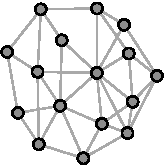
\includegraphics[width=.33\textwidth]{homophNet} & \hspace{2cm} &
	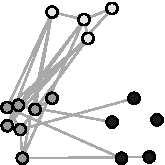
\includegraphics[width=.33\textwidth]{stochEquivNet}	
	\end{tabular}
	\label{fig:homphStochEquivNet}
\end{figure}

Another third-order dependence pattern that cannot be accounted for in the additive effects framework is stochastic equivalence. A pair of actors $ij$ are stochastically equivalent if the probability of $i$ relating to, and being related to, by every other actor is the same as the probability for $j$. This refers to the idea that there will be groups of nodes in a network with similar relational patterns. The occurrence of a dependence pattern such as this is not uncommon in the social science applications. Recent work estimates a stochastic equivalence structure to explain the formation of preferential trade agreements (PTAs) between countries \cite{manger:etal:2012}. Specifically, they suggest that PTA formation is related to differences in per capita income levels between countries. Countries falling into high, middle, and low income per capita levels will have patterns of PTA formation that are determined by the groups into which they fall. Such a structure is represented in the right-most panel of Figure~\ref{fig:homphStochEquivNet}, here the lightly shaded group of nodes at the top can represent high-income countries, nodes on the bottom-left middle-income, and the darkest shade of nodes low-income countries. The behavior of actors in a network can at times be governed by group level dynamics, and failing to account for such dynamics leaves potentially important parts of the data generating process ignored.

To account for third-order dependence patterns within the context of the SRRM we turn to latent variable models, which have become a popular approach for modeling relational data in fields as diverse as biology to computer science to the social sciences. These models assumes that relationships between nodes are mediated by a small number ($K$) of node-specific unobserved latent variables. One reason for their increased usage is that they enable researchers to capture and visualize third-order dependencies in a way that other approaches are not able to replicate. %Additionally, the conditional independence assumption facilitates the testing of a variety of nodal and dyadic level theories, and provides a range of computational advantages relative to ERGMs.

A number of latent variable approaches have been developed to represent third-order dependencies in relational data, we focus on two here: the the latent distance model
(LDM) and the latent factor model (LFM). For the sake of exposition, we consider the case where relations are symmetric to describe the differences between these approaches. Both of these approaches can be incorporated into an asymmetric version of the framework that we have been constructing through the inclusion of an additional term to the model for $y_{ij}$, $\alpha(u_{i}, u_{j})$, that captures latent third-order characteristics of a network, where $u_{i}$ and $u_{j}$ are node-specific latent variables. General definitions for how $\alpha(u_{i}, u_{j})$ is defined for these latent variable models are shown in Equations~\ref{eqn:latAlpha}. One other point of note about these approaches is that researchers have to specify a value for $K$.
%In the case of the latent distance and factor models, a value of $K$ equal to two or three is typically large enough to account for third-order dependencies in relational data.
These two approaches are given below:

\begin{align}
\begin{aligned}
\text{Latent distance model} \\
	&\alpha(\textbf{u}_{i}, \textbf{u}_{j}) = -|\textbf{u}_{i} - \textbf{u}_{j}| \\
	&\textbf{u}_{i} \in \mathbb{R}^{K}, \; i \in \{1, \ldots, n \} \\
\text{Latent factor model} \\
	&\alpha(\textbf{u}_{i}, \textbf{u}_{j}) = \textbf{u}_{i}^{\top} \Lambda \textbf{u}_{j} \\
	&\textbf{u}_{i} \in \mathbb{R}^{K}, \; i \in \{1, \ldots, n \} \\
	&\Lambda \text{ a } K \times K \text{ diagonal matrix}
\label{eqn:latAlpha}
\end{aligned}
\end{align}

In the LDM approach introduced in \cite{hoff:etal:2002}, each node $i$ has some unknown latent position in $K$ dimensional space, $\textbf{u}_{i} \in \mathbb{R}^{K}$, and the probability of a tie between a pair $ij$ is a function of the negative Euclidean distance between them: $-|\textbf{u}_{i} - \textbf{u}_{j}|$. Because latent distances for a triple of actors obey the triangle inequality, this formulation models the tendencies toward homophily commonly found in social networks. This approach is implemented in the \pkg{latentnet} which is part of the \pkg{statnet} $\sf{R}$ package \cite{krivitsky:handcock:2015}. However, this approach also comes with an important shortcoming: it confounds stochastic equivalence and homophily. Consider two nodes $i$ and $j$ that are proximate to one another in $K$ dimensional Euclidean space, this suggests not only that $|\textbf{u}_{i} - \textbf{u}_{j}|$ is small but also that $|\textbf{u}_{i} - \textbf{u}_{l}| \approx |\textbf{u}_{j} - \textbf{u}_{l}|$, the result being that nodes $i$ and $j$ will by construction assumed to possess the same relational patterns with other actors such as $l$ (i.e., that they are stochastically equivalent). Thus LDMs confound strong ties with stochastic equivalence. This approach cannot adequately model data with many ties between nodes that have different network roles.

This is problematic as real-world networks exhibit varying degrees of stochastic equivalence and homophily. In these situations, using the LDM would end up representing only a part of the network structure. In the latent factor model, each actor has an unobserved vector of characteristics, $\textbf{u}_{i} = \{u_{i,1}, \ldots, u_{i,K} \}$, which describe their behavior as an actor in the network. The probability of a tie from $i$ to $j$ depends on the extent to which $\textbf{u}_{i}$ and $\textbf{u}_{j}$ are ``similar'' (i.e., point in the same direction) and on whether the entries of $\Lambda$ are greater or less than zero.

% The singular value decomposition is a model based analogue to the eigenvalue decomposition for directed networks.
More specifically, the similarity in the latent factors, $\textbf{u}_{i} \approx \textbf{u}_{j}$, corresponds to how stochastically equivalent a pair of actors are and the eigenvalue determines whether the network exhibits positive or negative homophily. For example, say that we estimate a rank-one latent factor model (i.e., $K=1$), in this case $\textbf{u}_{i}$ is represented by a scalar $u_{i,1}$, similarly, $\textbf{u}_{j}=u_{j,1}$, and $\Lambda$ will have just one diagonal element $\lambda$. The average effect this will have on $y_{ij}$ is simply $\lambda \times u_{i} \times u_{j}$, where a positive value of $\lambda>0$ indicates homophily and $\lambda<0$ anti-homophily. This approach can represent both homophily and stochastic equivalence, and that the alternative latent variable approaches can be represented as a latent factor model but not vice versa \cite{hoff:2008}. In the directed version of this approach, we use the singular value decomposition, here actors in the network have a vector of latent characteristics to describe their behavior as a sender, denoted by $\textbf{u}$, and as a receiver, $\textbf{v}$: $\textbf{u}_{i}, \textbf{v}_{j} \in \mathbb{R}^{K}$. This can alter the probability of an interaction between $ij$ additively: $\textbf{u}_{i}^{\top} \textbf{D} \textbf{v}_{j}$, where $\textbf{D}$ is a $K \times K$ diagonal matrix.

Both the latent distance and factor models are ``conditional independence models'' in that they assume that ties are conditionally independent given all of the observed predictors and unknown node-specific parameters: $p( Y | X , U ) = \prod_{i<j} p( y_{i,j}  | x_{i,j} , u_i , u_j)$. Typical parametric models of this form relate $y_{i,j}$ to $(x_{i,j},u_i,u_j)$ via some sort of link function:

\begin{align*}
	p(y_{i,j} | x_{i,j}, u_i , u_j ) & = f( y_{i,j} : \eta_{i,j} ) \\
	\eta_{i,j} &= \beta^\top x_{i,j} + \alpha(\textbf{u}_{i}, \textbf{u}_{j}).
\end{align*}

The structure of $\alpha(\textbf{u}_{i}, \textbf{u}_{j})$ can result in very different interpretations for any estimates of the regression coefficients $\beta$. For example, suppose the latent effects $\{ u_1,\ldots, u_n\}$ are near zero on average (if not, their mean can be absorbed into an intercept parameter and row and column additive effects). Under the LFM, the average value of $\alpha(\textbf{u}_{i}, \textbf{u}_{j}) = \textbf{u}_{i}^{\top} \Lambda \textbf{u}_{j}$ will be near zero and so we have

\begin{align*}
	\eta_{i,j} & =  \beta^\top x_{i,j} + \textbf{u}_{i}^{\top} \Lambda \textbf{u}_{j} \\
	\bar \eta & \approx  \beta^\top \bar x.
\end{align*}

The implication of this is that the values of $\beta$ can be interpreted as yielding the ``average'' value of $\eta_{i,j}$. On the other hand, under the LDM

\begin{align*}
	\eta_{i,j} & =  \beta^\top x_{i,j} - |\textbf{u}_{i} - \textbf{u}_{j}|  \\
	\bar \eta & \approx  \beta^\top \bar x - \overline{ |\textbf{u}_{i} - \textbf{u}_{j}| } <  \beta^\top \bar x .
\end{align*}

In this case, $\beta^\top \bar x$ does not represent an ``average'' value of the predictor $\eta_{i,j}$, it represents a maximal value as if all actors were zero distance from each other in the latent social space. For example, consider the simplest case of a normally distributed network  outcome with an identity link. In this case,

\begin{align*}
	y_{i,j} & = \beta^\top x_{i,j} + \alpha(\textbf{u}_{i}, \textbf{u}_{j}) + \epsilon_{i,j} \\
	\bar y & \approx \beta^\top \bar x + \overline{ \alpha(\textbf{u}_{i}, \textbf{u}_{j}) }   .
\end{align*}

Under the LDM, $\bar y \approx \beta^\top \bar x + \overline{ |\textbf{u}_{i} - \textbf{u}_{j}|  } < \beta^\top \bar x$, and so we no longer can interpret $\beta$ as representing the linear relationship between $y$ and $x$. Instead, it may be thought of as describing some sort of average hypothetical ``maximal'' relationship between $y_{i,j}$ and $x_{i,j}$.

Thus the LFM provides two important benefits. First, we are able to capture a wider assortment of dependence patterns that arise in relational data, and, second, parameter interpretation is more straightforward. The AME approach considers the regression model shown in Equation~\ref{eqn:ame}:

\begin{align}
\begin{aligned}
	y_{ij} &= g(\theta_{ij}) \\
	&\theta_{ij} = \bm\beta^{\top} \mathbf{X}_{ij} + e_{ij} \\
	&e_{ij} = a_{i} + b_{j}  + \epsilon_{ij} + \alpha(\textbf{u}_{i}, \textbf{v}_{j}) \text{  , where } \\
	&\qquad \alpha(\textbf{u}_{i}, \textbf{v}_{j}) = \textbf{u}_{i}^{\top} \textbf{D} \textbf{v}_{j} = \sum_{k \in K} d_{k} u_{ik} v_{jk}. \\
\label{eqn:ame}
\end{aligned}
\end{align}

Using this framework, we are able to model the dyadic observations as conditionally independent given $\bm\theta$, where $\bm\theta$ depends on the the unobserved random effects, $\mathbf{e}$. $\mathbf{e}$ is then modeled to account for the potential first, second, and third-order dependencies that we have discussed. As described in Equation~\ref{eqn:srmCov}, $a_{i} + b_{j}  + \epsilon_{ij}$, are the additive random effects in this framework and account for sender, receiver, and within-dyad dependence. The multiplicative effects, $\textbf{u}_{i}^{\top} \textbf{D} \textbf{v}_{j}$, are used to capture higher-order dependence patterns that are left over in $\bm\theta$ after accounting for any known covariate information. %A Bayesian procedure in which parameters are iteratively updated using a Gibbs sampler is available in an $\sf{R}$ package.%\footnote{The set of parameters that are estimated in the model from the observed data, $\{\mathbf{Y}, \mathbf{X}\}$, are: latent Gaussian variables ($\bm\theta$); nodal and/or dyadic regression coefficients ($\bm\beta$); additive nodal random effects ($\{(a_{i},b_{i})\} \in \{i=1, \ldots, n \}$); network covariance ($\Sigma_{ab},\, \Sigma_{\epsilon}$); multiplicative effects ($\mathbf{U}$, $\mathbf{V}$, and $\mathbf{D}$).}

\section*{\textbf{ERGMs}}

An alternative approach to accounting for third-order dependence patterns are ERGMs. This approach was first developed by \citet{erdos:renyi:1959}, and has became more widely understood as it has been applied to particular problems. \citet{frank:1971} undertook an early examination and Julian Besag developed interesting applications and methods promoting their examination (\citealt{besag:1977b}). But obtaining estimates was computational challenging and it was not until \citet{frank:strauss:1986} and \citet{wasserman:pattison:1996} that these methods found widespread application. These so-called ERGM approaches are particularly useful when researchers are interested in the role that a specific list of network statistics have in giving rise to a certain network. These network statistics could include the number of transitive triads in a network, balanced triads, reciprocal pairs and so on.\footnote{\citet{morris:etal:2008} and \citet{snijders:etal:2006} provide a detailed list of network statistics that can be included in an ERGM model specification.} In the ERGM framework, a set of statistics, $S(\mathbf{Y})$, define a model. Given the chosen set of statistics, the probability of observing a particular network dataset $\mathbf{Y}$ can be expressed as:

\begin{align}
\Pr(Y = y) = \frac{ \exp( \bm\beta^{\top} S(y)  )  }{ \sum_{z \in \mathcal{Y}} \exp( \bm\beta^{\top} S(z)  )  } \text{ ,  } y \in \mathcal{Y}.
\label{eqn:ergm}
\end{align}

$\bm\beta$ represents a vector of model coefficients for the specified network statistics, $\mathcal{Y}$ denotes the set of all obtainable networks, and the denominator is used as a normalizing factor (\citealt{hunter:etal:2008}). This approach provides a way to state that the probability of observing a given network depends on the patterns that it exhibits, which are operationalized in the list of network statistics specified by the researcher. Within this approach one can test the role that a variety of network statistics play in giving rise to a particular network.

One issue that arises when conducting statistical inference with this model is in the calculation of the normalizing factor, which is what ensures that the expression above corresponds to a legitimate probability distribution. For even a trivially sized directed network that has only $20$ actors, calculating the denominator means summing over $2^{20\times(20-1)} = 2^{380}$ possible networks, or, to put it another way, more than the total number of atoms in the universe. One of the first approaches to deal with this issue was a computationally fast pseudo-likelihood approach developed by Strauss \& Ikeda (\citealt{strauss:ikeda:1990}). However, this approach ignores the interdependent nature of observations in relational data, as a result, many have argued that the standard errors remain unreliable (\citealt{vanduijn:etal:2009}). Additionally, there is no asymptotic theory underlying this approach on which to base the construction of confidence intervals and hypothesis tests (\citealt{kolaczyk:2009}). The pseudo-likelihood approach has became increasingly unpopular in recent years among those in the network analysis community, particularly, as simulation based techniques have developed--though it has not disappeared. One favored approach in the literature is to approximate the MLE using Markov Chain Monte Carlo techniques, also referred to as MCMC-MLE (\citealt{geyer:thompson:1992,snijders:2002,handcock:2003a}).

The MCMC-MLE approach is an advancement but notable problems remain. Unlike latent variable models, Rastelli et al. (\citealt{rastelli:etal:2016}) argue that ERGMs are not even able to represent transitivity asymptotically as their clustering coefficient converges to zero. Chatterjee \& Diaconis (\citealt{chatterjee:diaconis:2013}) have shown that MCMC procedures can take an exponential time to converge for broad classes of ERGMs unless the dyadic observations are independent. This is a result of the fact that MCMC procedures visit an infinitesimally small portion of the set of possible graphs. A related issue when estimating ERGMs is that the estimated model can become degenerate even if the observed graph is not degenerate. This means that the model is placing a large amount of probability on a small subset of networks that fall in the set of obtainable networks, $\mathcal{Y}$, but share little resemblance with the observed network (\citealt{schweinberger:2011}). For example, most of the probability may be placed on empty graphs, no edges between nodes, or nearly complete graphs, almost every node is connected by an edge. Some have argued that model degeneracy is simply a result of model misspecification (\citealt{goodreau:etal:2008,handcock:etal:2008}). This points to an important caveat in interpreting the implications of an often cited basis for ERGM, the Hammersley-Clifford theorem. Though this theorem ensures that any network can be represented through an ERGM, it says nothing about the complexity of the sufficient statistics ($S(y)$) required to do so. Failure to properly account for higher-order dependence structures through an appropriate specification can at best lead to model degeneracy, which provides an obvious indication that the specification needs to be altered, and at worst deliver a result that converges but does not appropriately capture the interdependencies in the network. The consequence of the latter case is a set of inferences that will continue to be biased as a result of unmeasured heterogeneity, thus defeating the major motivation for pursuing an inferential network model in the first place. 

In the following section we undertake a comparison of the latent distance model, ERGM, and the AME model. In doing so, we are able to compare and contrast these various approaches.

\section*{\textbf{Empirical Comparison}}

To contrast AME with these alternative approaches, we utilize a cross-sectional network measuring whether an actor indicated that they collaborated with each other during the policy design of the Swiss CO$_{2}$ act (\citealt{ingold:2008}). This is a directed relational matrix as an actor $i$ can indicate that they collaborated with $j$ but $j$ may not have stated that they collaborated with $i$. The Swiss government proposed this act in 1995 with the goal of undertaking a 10\% reduction in CO$_{2}$ emissions by 2012. The act was accepted in the Swiss Parliament in 2000 and implemented in 2008. Ingold \cite{ingold:2008}, and subsequent work by Ingold \& Fischer \cite{ingold:fischer:2014}, sought to determine what drives collaboration among actors trying to affect climate change policy. The set of actors included in this network are those that were identified by experts as holding an important position in Swiss climate policy. In total, Ingold identifies 34 relevant actors: five state actors, eleven industry and business representatives, seven environmental NGOs and civil society organizations, five political parties, and six scientific institutions and consultants. We follow Ingold \& Fischer and Cranmer et al. \cite{cranmer:etal:2016} in developing a model specification to understand and predict link formation in this network.\footnote{We do not review the specification in detail here, instead we just provide a summary of the variables to be included and the theoretical expectations of their effects in the Appendix.}

The LDM we fit on this network includes a two-dimensional Euclidean distance metric. The ERGM specification for this network includes the same exogenous variables as LDM, but also includes a number of endogenous characteristics of the network. The AME model we fit here includes the same exogenous covariates and accounts for nodal and dyadic heterogeneity using the SRM. Third-order effects are represented by the latent factor model with $K=2$. Parameter estimates for these three approaches are shown in Table~\ref{tab:regTable}.

The first point to note is that, in general, the parameter estimates returned by the AME are similar to those of ERGM but quite different from the LDM. For example, while the LDM returns a result for the \texttt{Opposition/alliance} variable that diverges from ERGM, the AME returns a result that is similar to Ingold \& Fischer. Similar discrepancies appear for other parameters such as \texttt{Influence attribution} and \texttt{Alter's influence degree}. Each of these discrepancies are eliminated when using AME. As described previously, this is because the LDM approach complicates the interpretation of the effects of exogenous variables.\footnote{In the SI Appendix, we show that these differences persist even when incorporating sender and receiver random effects.}

% latex table generated in R 3.3.1 by xtable 1.8-2 package
% Sun Aug 21 03:32:43 2016
\begin{table}[ht]
\centering
\caption{* p $<$ 0.05. ERGM results are shown with standard errors in parentheses. LDM and AME are shown with 95\% posterior credible intervals provided in brackets.}
\begin{tabular}{lccc}
  & LDM & ERGM & AME \\
  \hline
\hline
Intercept/Edges & 0.94$^{\ast}$ & -12.17$^{\ast}$ & -3.39$^{\ast}$ \\
   & [0.09; 1.82] & (1.40) & [-4.38; -2.50] \\
  \textbf{Conflicting policy preferences}  &  &  &  \\
  $\;\;\;\;$ Business vs. NGO & -1.37$^{\ast}$ & -1.11$^{\ast}$ & -1.37$^{\ast}$ \\
   & [-2.42; -0.41] & (0.51) & [-2.44; -0.47] \\
  $\;\;\;\;$ Opposition/alliance  & 0.00 & 1.22$^{\ast}$ & 1.08$^{\ast}$ \\
   & [-0.40; 0.39] & (0.20) & [0.72; 1.47] \\
  $\;\;\;\;$ Preference dissimilarity & -1.76$^{\ast}$ & -0.44 & -0.79$^{\ast}$ \\
   & [-2.62; -0.90] & (0.39) & [-1.55; -0.08] \\
  \textbf{Transaction costs}  &  &  &  \\
  $\;\;\;\;$ Joint forum participation & 1.51$^{\ast}$ & 0.90$^{\ast}$ & 0.92$^{\ast}$ \\
   & [0.86; 2.17] & (0.28) & [0.40; 1.47] \\
  \textbf{Influence}  &  &  &  \\
  $\;\;\;\;$ Influence attribution & 0.08 & 1.00$^{\ast}$ & 1.09$^{\ast}$ \\
   & [-0.40; 0.55] & (0.21) & [0.69; 1.53] \\
  $\;\;\;\;$ Alter's influence indegree & 0.01 & 0.21$^{\ast}$ & 0.11$^{\ast}$ \\
   & [-0.03; 0.04] & (0.04) & [0.07; 0.15] \\
  $\;\;\;\;$ Influence absolute diff. & 0.04 & -0.05$^{\ast}$ & -0.07$^{\ast}$ \\
   & [-0.01; 0.09] & (0.01) & [-0.11; -0.03] \\
  $\;\;\;\;$ Alter = Government actor & -0.46 & 1.04$^{\ast}$ & 0.55 \\
   & [-1.08; 0.14] & (0.34) & [-0.07; 1.15] \\
  \textbf{Functional requirements}  &  &  &  \\
  $\;\;\;\;$ Ego = Environmental NGO & -0.60 & 0.79$^{\ast}$ & 0.67 \\
  & [-1.32; 0.09] & (0.17) & [-0.38; 1.71] \\
  $\;\;\;\;$ Same actor type & 1.17$^{\ast}$ & 0.99$^{\ast}$ & 1.04$^{\ast}$ \\
   & [0.63; 1.71] & (0.23) & [0.63; 1.50] \\
  \textbf{Endogenous dependencies}  &  &  &  \\
  $\;\;\;\;$ Mutuality &  & 0.81$^{\ast}$ & 0.39 \\
   &  & (0.25) & [-0.12; 0.96] \\
  $\;\;\;\;$ Outdegree popularity  &  & 0.95$^{\ast}$ &  \\
   &  & (0.09) &  \\
  $\;\;\;\;$ Twopaths  &  & -0.04$^{\ast}$ &  \\
  &  & (0.02) &  \\
  $\;\;\;\;$ GWIdegree (2.0)  &  & 3.42$^{\ast}$ &  \\
   &  & (1.47) &  \\
  $\;\;\;\;$ GWESP (1.0)  &  & 0.58$^{\ast}$ &  \\
   &  & (0.16) &  \\
  $\;\;\;\;$ GWOdegree (0.5)  &  & 8.42$^{\ast}$ &  \\
   &  & (2.11) &  \\
   \hline
\hline
\end{tabular}
\label{tab:regTable}
\end{table}
\FloatBarrier

There are also a few differences between the parameter estimates that result from the ERGM and AME. Using the AME we find evidence that \texttt{Preference dissimilarity} is associated with a reduced probability of collaboration between a pair of actors, which is in line with the theoretical expectations of Ingold \& Fischer. Additionally, the AME results differ from ERGM for the nodal effects related to whether a receiver of a collaboration is a government actor, \texttt{Alter=Government actor}, and whether the sender is an environmental NGO, \texttt{Ego=Environmental NGO}.

\subsection*{Tie Formation Prediction}

Next, we utilize a cross-validation procedure to assess the out-of-sample performance for each of the models presented in Table~\ref{tab:regTable} as follows:

\begin{itemize}
	\item Randomly divide the $n \times (n-1)$ data points into $S$ sets of roughly equal size, letting $s_{ij}$ be the set to which pair $\{ij\}$ is assigned.
	\item For each $s \in \{1, \ldots, S\}$:
	\begin{itemize}
		\item Obtain estimates of the model parameters conditional on $\{y_{ij} : s_{ij} \neq s\}$, the data on pairs not in set $s$.
		\item For pairs $\{kl\}$ in set $s$, let $\hat y_{kl} = E[y_{kl} | \{y_{ij} : s_{ij} \neq s\}]$, the predicted value of $y_{kl}$ obtained using data not in set $s$.
	\end{itemize}
\end{itemize}

The procedure summarized in the steps above generates a sociomatrix of out-of-sample predictions of the observed data. Each entry $\hat y_{ij}$ is a predicted value obtained from using a subset of the data that does not include $y_{ij}$. In this application we set $S$ to 45 which corresponds to randomly excluding approximately 2\% of the data from the estimation. Such a low number of observations were excluded in every sample (denoted a fold) because excluding any more observations would cause the ERGM specification to result in a degenerate model that empirically can not be fit. This highlights the computational difficulties associated with ERGMs in the presence of even small amounts of missing data.

Using the set of out-of-sample predictions we generate from the cross-validation procedure, we provide a series of tests to assess model fit. The left-most plot in Figure~\ref{fig:roc} compares the five approaches in terms of their ability to predict the out-of-sample occurrence of collaboration based on Receiver Operating Characteristic (ROC) curves. ROC curves provide a comparison of the trade-off between the True Positive Rate (TPR), sensitivity, False Positive Rate (FPR), 1-specificity, for each model. Models that have a better fit according to this test should have curves that follow the left-hand border and then the top border of the ROC space. On this diagnostic, the AME model performs best closely followed by ERGM. The LDM approach lags notably behind the other specifications. 

A more intuitive visualization of the differences between these modeling approaches can be gleaned through examining the separation plots included on the right-bottom edge of the ROC plot. This visualization tool plots each of the observations, in this case actor pairs, in the dataset according to their predicted value from left (low values) to right (high values). Models with a good fit should have all network links, here these are colored by the modeling approach, towards the right of the plot. Using this type of visualization emphasizes that the AME and ERGM models performs better than the latent distance approach.

\begin{figure}[ht]
	\centering
	\caption{Assessments of out-of-sample predictive performance using ROC curves, separation plots, and PR curves. AUC statistics are also provided.}
	\begin{tabular}{cc}
	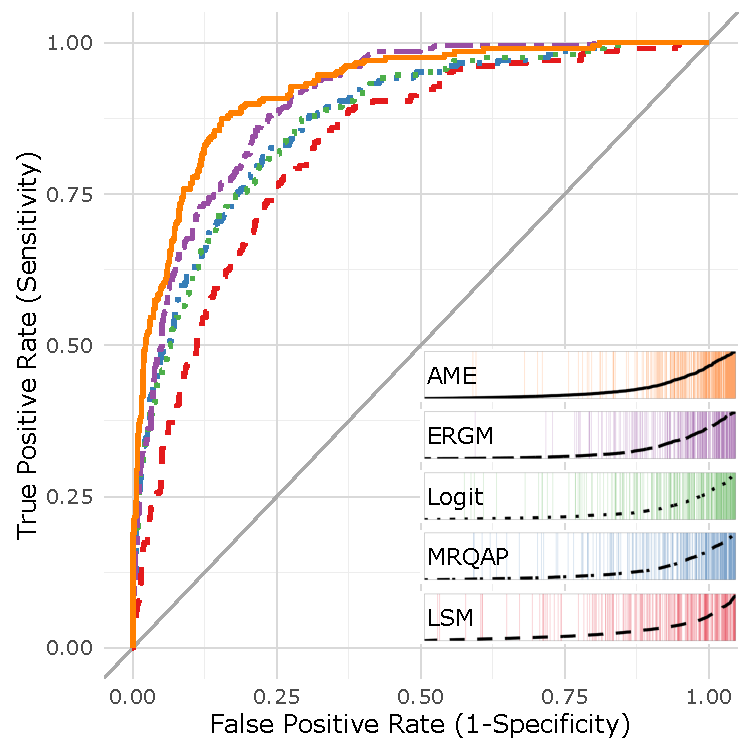
\includegraphics[width=.5\textwidth]{roc_outSample} & 
	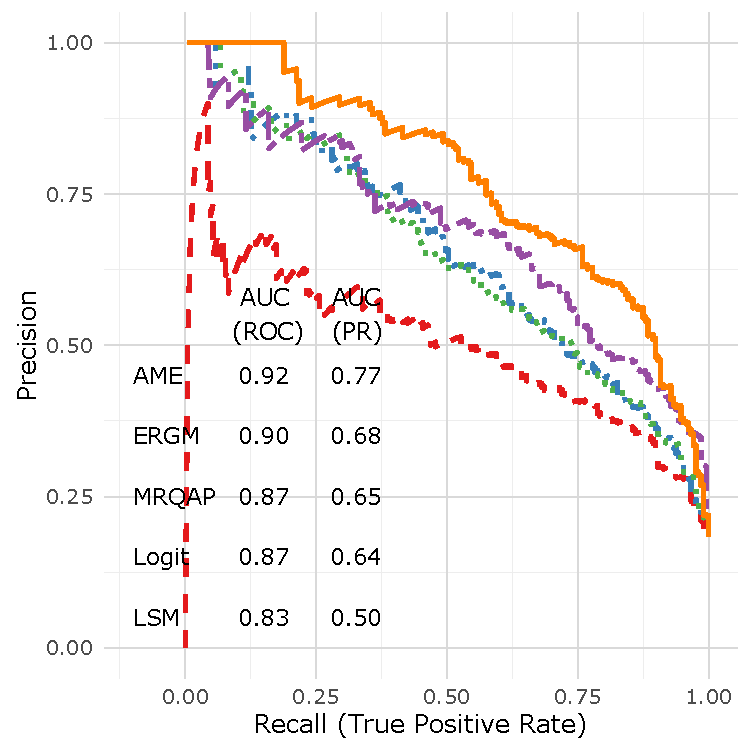
\includegraphics[width=.5\textwidth]{rocPr_outSample}	
	\end{tabular}
	\label{fig:roc}
\end{figure}

The last diagnostic we highlight to assess predictive performance are precision-recall (PR) curves. In both ROC and PR space we utilize the TPR, also referred to as recall--though in the former it is plotted on the y-axis and the latter the x-axis. The difference, however, is that in ROC space we utilize the FPR, while in PR space we use precision. FPR measures the fraction of negative examples that are misclassified as positive, while precision measures the fraction of examples classified as positive that are truly positive. PR curves are useful in situations where correctly predicting events is more interesting than simply predicting non-events (\citealt{davis:goadrich:2006}). This is especially relevant in the context of studying many relational datasets in political science such as conflict, because events in such data are extremely sparse and it is relatively easy to correctly predict non-events. In the case of our application dataset, the vast majority of dyads, 80\%, do not have a network linkage, which points to the relevance of assessing performance using the PR curves as we do in the right-most plot of Figure~\ref{fig:roc}. We can see that the relative-ordering of the models remains similar but the differences in how well they perform become much more stark. Here we find that the AME approach performs notably better in actually predicting network linkages than each of the alternatives. Area under the curve (AUC) statistics are provided in Figure~\ref{fig:roc} and these also highlight AME's superior out-of-sample performance.


\FloatBarrier

\subsection*{Capturing Network Attributes}

We also assess which of these models best captures the network features of the dependent variable. To do this, we compare the observed network with a set of networks simulated from the estimated models. We simulate 1,000 networks from the three models and compare how well they align with the observed network in terms of four network statistics: (1) the empirical standard deviation of the row means (i.e., heterogeneity of nodes in terms of the ties they send); (2) the empirical standard deviation of the column means (i.e., heterogeneity of nodes in terms of the ties they receive); (3) the empirical within-dyad correlation (i.e., measure of reciprocity in the network); and (4) a normalized measure of triadic dependence. A comparison of the LDM, ERGM, and AME models among these four statistics is shown in Figure~\ref{fig:ergmAmePerf}.\footnote{In the SI Appendix, we compare the ability of these models to capture network attribute across a wider array of statistics, and the results are consistent with what we present below.}

\begin{figure}[ht]
	\centering
	\caption{Network goodness of fit summary using \pkg{amen}.}
	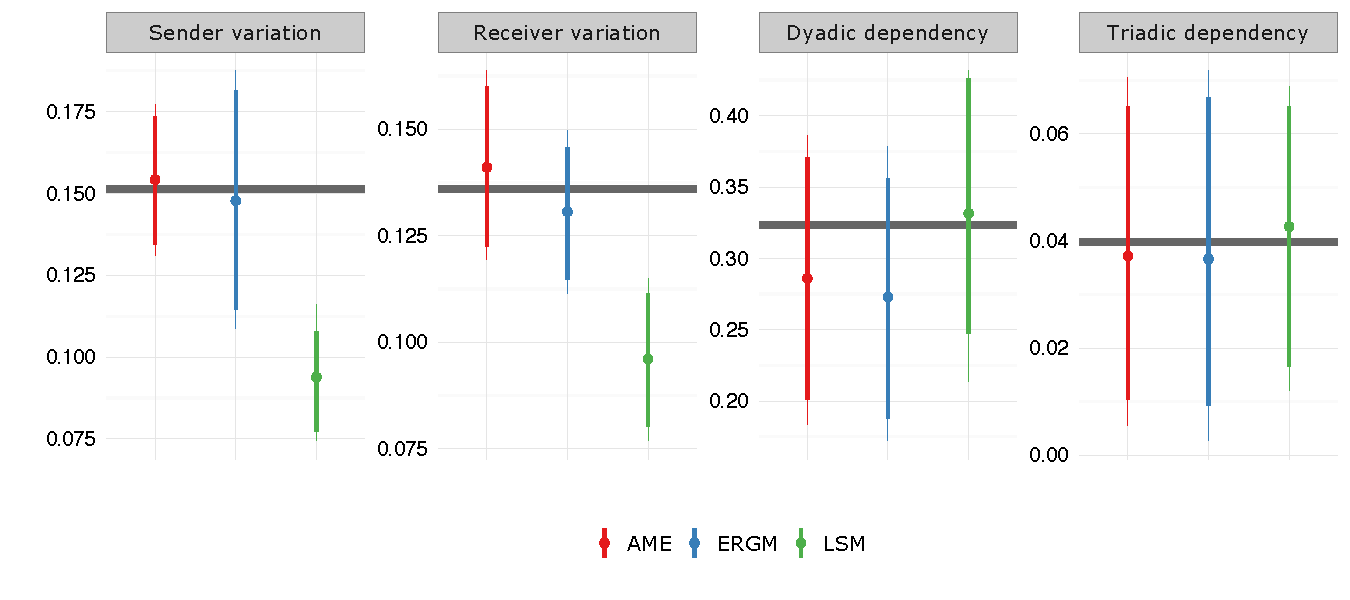
\includegraphics[width=1\textwidth]{netPerfCoef}
	\label{fig:ergmAmePerf}
\end{figure}
\FloatBarrier

Here it becomes quickly apparent that the LDM model fails to capture how active and popular actors are in the Swiss climate change mitigation network.\footnote{Further even after incorporating random sender and receiver effects into the LDM framework this problem is not completely resolved, see the SI Appendix for details.} The AME and ERGM specifications again both tend to do equally well. If when running this diagnostic, we found that the AME model did not adequately represent the observed network this would indicate that we might want to increase $K$ to better account for network interdependencies. No changes to the model specification as described by the exogenous covariates a researcher has chosen would be necessary. If the ERGM results did not align with the diagnostic presented in Figure~\ref{fig:ergmAmePerf}, then this would indicate that an incorrect set of endogenous dependencies have been specified. Failing to identify (or find) the right specification will leave the researcher with the problems we introduced earlier.

\section*{\textbf{Conclusion}}

The AME approach to estimation and inference in network data provides a number of benefits over alternative approaches. Specifically, it provides a modeling framework for dyadic data that is based on familiar statistical tools such as linear regression, GLM, random effects, and factor models. We have an understanding of how each of these tools work, they are numerically more stable than ERGM approaches, and more general than alternative latent variable models. Further the estimation procedure utilized in AME avoids complicating interpretation of parameter estimates for exogenous variables. For researchers in the social sciences this is of primary interest, as many studies that employ relational data still have conceptualizations that are monadic or dyadic in nature. Additionally, through the application dataset utilized herein we show that the AME approach outperforms both ERGM and LDM in out-of-sample prediction, and also is better able to capture network dependencies than the LDM.

More broadly, relational data structures are composed of actors that are part of a system. It is unlikely that this system can be viewed simply as a collection of isolated actors or pairs of actors. The assumption  that dependencies between observations occur can at the very least be examined. Failure to take into account interdependencies leads to biased parameter estimates and poor fitting models. By using standard diagnostics such as shown in Figure~\ref{fig:ergmAmePerf}, one can easily assess whether an assumption of independence is reasonable. We stress this point because a common misunderstanding that seems to have emerged within the social science literature relying on dyadic data is that a network based approach is only necessary if one has theoretical explanations that extend beyond the dyadic. This is not at all the case and findings that continue to employ a dyadic design may misrepresent the effects of the very variables that they are interested in. The AME approach that we have detailed here provides a statistically familiar way for scholars to account for unobserved network structures in relational data. Additionally, through this approach we can visualize these dependencies in order to better learn about the network patterns that remain in the event of interest after having accounted for observed covariates.

When compared to other network based approaches, AME is easier to specify and utilize. It is also more straightforward to interpret since it does not require interpretation of unusual features such as \textit{three-stars} which fall outside of the normal language for discussing social science. Further, the \pkg{amen} package facilitates the modeling of longitudinal network data. In sum, excuses for continuing to treat relational data as conditionally independent are becoming increasingly harder to make.

\newpage

% Bib stuff
\clearpage
\bibliography{/Users/s7m/whistle/master}
% \bibliography{/Users/mdw/git/whistle/master}
% \bibliographystyle{elsarticle-harv}\biboptions{authoryear}
\bibliographystyle{APSR}\biboptions{authoryear}
\newpage

\end{document}